% Origen móvil: qué años entrenan y cuál se predice en cada corrida.
% Protocolo de notebooks/02_modelado.ipynb (sección 6).
\documentclass[border=2pt]{standalone}
% Estilo común de los diagramas: letra sin serifa, como las figuras del
% notebook, y ancho máximo de una columna IEEE (8,9 cm). Compilar con pdflatex.
\usepackage[utf8]{inputenc}
\usepackage[T1]{fontenc}
\usepackage{tgheros}
\renewcommand{\familydefault}{\sfdefault}
\usepackage{tikz}
\usetikzlibrary{positioning, arrows.meta, fit, backgrounds, calc}

\definecolor{pm}{HTML}{1F77B4}
\definecolor{meteo}{HTML}{2CA02C}
\definecolor{modelo}{HTML}{FF7F0E}
\definecolor{perdida}{HTML}{B22222}
\definecolor{gris}{HTML}{6E6E6E}

\tikzset{
  caja/.style={draw=#1, fill=#1!8, rounded corners=2pt, line width=0.6pt,
    align=center, inner sep=3pt, font=\fontsize{6.5}{7.8}\selectfont},
  caja/.default=gris,
  flecha/.style={-{Stealth[length=4pt]}, line width=0.6pt, draw=gris},
  nota/.style={font=\fontsize{5.8}{7}\selectfont, text=perdida, align=left},
  titulo/.style={font=\fontsize{6.5}{7.8}\selectfont\bfseries, text=#1},
}
\newcommand{\menos}[1]{\textcolor{perdida}{\fontsize{5.8}{7}\selectfont #1}}


\begin{document}
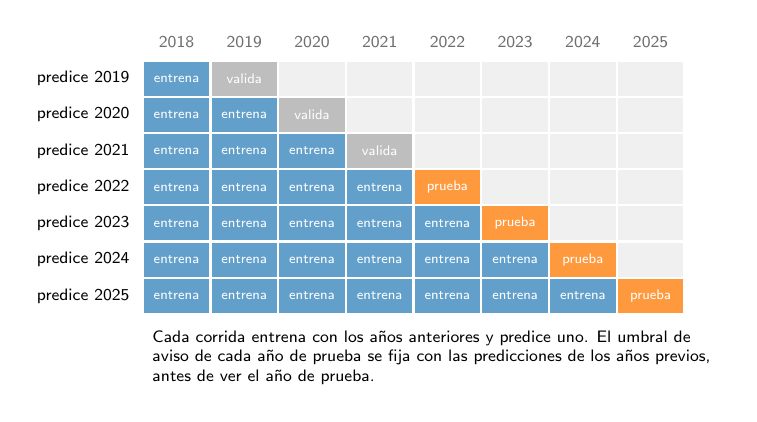
\begin{tikzpicture}[x=8.6mm, y=-4.6mm,
    celda/.style={draw=white, line width=0.8pt, minimum width=8.6mm, minimum height=4.6mm,
      inner sep=0pt, font=\fontsize{5.5}{6}\selectfont},
    etiqueta/.style={font=\fontsize{6}{7}\selectfont}]
  \foreach \c [count=\i from 0] in {2018,...,2025}
    \node[etiqueta, text=gris] at (\i+1, 0) {\c};
  \foreach \y [count=\r from 1] in {2019,...,2025} {
    \pgfmathtruncatemacro{\pred}{\y-2017}
    \ifnum\y<2022 \def\colorpred{gris!45}\def\textopred{valida}
    \else \def\colorpred{modelo!80}\def\textopred{prueba}\fi
    \node[etiqueta, anchor=east] at (0.45, \r) {predice \y};
    \foreach \i in {1,...,8} {
      \ifnum\i<\pred \node[celda, fill=pm!70, text=white] at (\i, \r) {entrena};
      \else\ifnum\i=\pred \node[celda, fill=\colorpred, text=white] at (\i, \r) {\textopred};
      \else \node[celda, fill=gris!10] at (\i, \r) {};
      \fi\fi
    }
  }
  \node[etiqueta, text width=72mm, align=flush left, anchor=north west] at (0.5, 7.7)
    {Cada corrida entrena con los años anteriores y predice uno. El umbral de
     aviso de cada año de prueba se fija con las predicciones de los años
     previos, antes de ver el año de prueba.};
\end{tikzpicture}
\end{document}
